\documentclass[11pt,a4paper]{article}

\usepackage{epsfig}
\usepackage{multicol}

\usepackage[utf8]{inputenc}
\usepackage[brazil]{babel}
\usepackage{fancyheadings}
\usepackage{amsmath}
\usepackage{calrsfs}
\usepackage{enumerate}
\usepackage{enumitem}   
\DeclareGraphicsExtensions{.png,.pdf}
\usepackage{amsmath, amsfonts, amssymb}
\usepackage{esint}
\usepackage{graphicx}
\usepackage{multicol}
\usepackage{tasks}
\usepackage[utf8]{inputenc}
\usepackage{mathrsfs} % Transformada de Laplace
\usepackage{indentfirst}

% As margens
\setlength{\textheight}{24.0cm}
\setlength{\textwidth}{17.5cm}
\setlength{\oddsidemargin}{2.0cm} % Margens reais desejadas
\setlength{\evensidemargin}{2.0cm} % 2+17.5+1.5=21cm (largura A4)
\setlength{\topmargin}{1.5cm} % 1.5+1.6+1.0+24.0+1.6=29.7cm
\setlength{\headheight}{1.6cm} % (altura A4)
\setlength{\headsep}{1.0cm}
\setlength{\columnsep}{1.5cm} % Coluna = 8cm ((17.5-1.5)/2)
\addtolength{\oddsidemargin}{-1in}
\addtolength{\evensidemargin}{-1in}
\addtolength{\topmargin}{-1in}
\setlength{\footskip}{0.0cm}


% Novos comandos
\newcommand{\limite}{\displaystyle\lim}
\newcommand{\integral}{\displaystyle\int}
\newcommand{\somatorio}{\displaystyle\sum}
\newcommand{\mat}[1]{\mbox{\boldmath{$#1$}}} 

\pagestyle{fancy}


\usepackage{lipsum}

\lhead{

\includegraphics[width=1cm]{brasao.png}
}

\rhead{ 
\sc\textbf{U}niversidade \textbf{F}ederal do \textbf{C}eará\\
Campus Quixadá\\ Eletricidade e Magnetismo}

\cfoot{}

\begin{document}

	\begin{center}
		\Large Mateus Sousa Araújo 
	\end{center}
	

	\begin{enumerate}
	
	\item Determine o fluxo do campo vetorial $F(x,y,z) = z\vec{i} + y\vec{j} + x\vec{k}$ sobre a unidade esférica $x^2 + y^2 + z^2 = 1$.
	
	\item Calcule $\displaystyle\iint_S F \cdot dS$, onde 
	$$F(x,y,z) = xy\vec{i} \, + (y^2 + e^{xz^2})\vec{j} \, + \sin (xy)\vec{k}$$
	E $S$ é a superfície da região $E$ delimitada pelo cilindro parabolóico $z = 1 - x^2$ e os planos $z = 0$, $y = 0$ e $y + z = 2$.
	
	\item O campo elétrico pode ser representado por 
	$$E(x) = \displaystyle\dfrac{\varepsilon Q}{|x|^3} x $$
	onde a carga elétrica $Q$ está localizada na origem e $x = \langle x \textrm{,}\ y \textrm{,}\ z \rangle$ é um vetor posição. Use o Teorema do Divergente para mostrar que o fluxo elétrico de $E$ através de qualquer superfície fechada $S_2$ que inclui a origem é
	$$\displaystyle\iint_{S_2} E \cdot dS = 4 \pi \varepsilon Q$$
	
	\item Calcule $\displaystyle\iint_C F \cdot dr$, onde $F(x,y,z) = -y^2\vec{i} + x\vec{j} + z^2\vec{k}$ e $C$ é a curva da intersecção do plano $y + z = 2$ com o cilindro $x^2 + y^2 = 1$. (Oriente $C$ no sentido anti-horário quando observado de cima.)
	
	
	
	\item Suponha que $S$ e $E$ satisfaçam as condições do Teorema do Divergente e que $f$ seja uma função escalar com derivadas parciais contínuas. Demonstre que
	$$\displaystyle\iint_S \ f \ n \ dS = \displaystyle\iiint_E \nabla f \ dV$$
	Estas integrais de superfície e triplas de funções vetoriais são vetores definidos por meio da integração de cada função do componente. [Dica: Comece por aplicar o Teorema do Divergente para $F = fc$, onde $c$ é um vetor constante arbitrário.]
	
	\item Seja $\vec{F}(x,y,z) = (x + y + z^2)\vec{k}$ e seja $\sigma$ a fronteira do cilindro $x^2 + y^2 \leq 4$ e $0 \leq z \leq 3$. Calcule $\displaystyle\iint_\sigma \vec{F} \cdot \vec{n} \, dS$ onde $\vec{n}$ é a normal exterior, isto é, $\vec{n}$ é a normal que aponta para fora do cilindro. 
 
	\item Seja $\vec{v}$ um campo vetorial de classe $C^1$ num aberto $\Omega$ de $\mathbb{R}^3$, com $\nabla \vec{v} = 0$ em $\Omega$. Seja $B \subset \Omega$ um compacto em forma de "tubo" ao qual o teorema da divergência se aplica. Sejam $\sigma_1$ e $\sigma_2$ as secções transversais, com normais $\vec{n_1}$ apontando para fora e $\vec{n_2}$ apontando para dentro de $B$. Suponha que $v$ seja tangente à superfície lateral do tubo. 
	
\begin{figure}[h]	
\centering % para centralizarmos a figura	
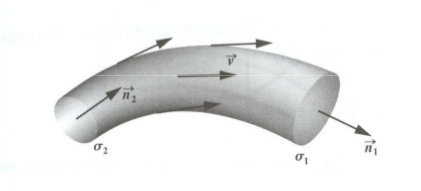
\includegraphics[width=6cm]{Selection_059.jpg} 
\end{figure}

Demonstre: 

$$\displaystyle\iint_{\sigma_1} \vec{v} \cdot \vec{n_1} \, dS = \displaystyle\iint_{\sigma_2} \vec{v} \cdot \vec{n_2} \, dS$$

\item Use o Teorema de Stokes para calcular a integral $\displaystyle\iint_S \nabla F \times  dS$, onde $F(x,y,z) = xz\vec{i} + yz\vec{j} + xy\vec{k}$ e $S$ é a parte da esfera $x^2 + y^2 + z^2 = 4$ que está dentro do cilindro $x^2 + y^2 = 1$ e acima do plano $xy$. 

\begin{figure}[h]	
\centering % para centralizarmos a figura	
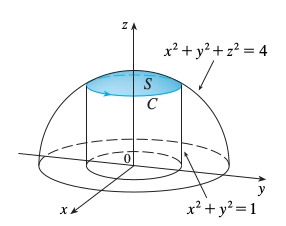
\includegraphics[width=5cm]{Selection_060.jpg} 
\end{figure}

\item Use o Teorema de Stokes para calcular $\displaystyle\iint_S \vec{\nabla} F \times  dS$.

\begin{enumerate}
\item $F(x,y,z) = (2y \cos z) \vec{i} + (e^x\sin z) \vec{j} + (xe^y) \vec{k}$, S é o hemisfério $x^2 + y^2 + z^2 = 9$, $z \geq 0$, de orientação ascendente. 
\item $F(x,y,z) = (x^2z^2)\vec{i} + (y^2z^2)\vec{i} + (xyz)\vec{k}$, S é a parte do paraboloide $z = x^2 + y^2$ que está dentro do cilindro $x^2 + y^2 = 4$, com orientação ascendente. 

\item $F(x,y,z) = (\arctan (x^2z^y2))\vec{i} + (x^2y)\vec{j} + (x^2z^2)\vec{k}$, S é o cone $x = \sqrt{y^2 - z^2}$, $0 \leq x \leq 2$, orientado na direção do eixo positivo x. 
\item $F(x,y,z) = (e^{xy})\vec{i} + (e^{xz})\vec{j} + (x^2z)\vec{k}$, S é a metdade do elipsoide $4x^2 + y^2 + 4z^2 = 4$ que se situa à direita do plano $xz$ orientado na direção do eixo positivo y. 
\end{enumerate}

\item Utilize os Teoremas de Gauss e Stokes e passe as Equações de Maxwell na forma integral abaixo

\begin{equation}
\oiint_{\partial V} \vec{E} \cdot \vec{n} \ ds  =\frac{Q_{int}}{\epsilon_0} 
\end{equation}

\begin{equation}
\oiint_{\partial V} \vec{B} \cdot \vec{n} \ ds  = 0  
\end{equation}

\begin{equation}
\ointctrclockwise_{\partial S} \vec{E} \cdot d\vec{r} = - \frac{\partial \phi _B }{\partial t}
\end{equation}

\begin{equation}
\ointctrclockwise_{\partial S} \vec{B} \cdot d\vec{r} = \mu_0i + \mu_0\varepsilon_0\frac{\partial \phi _E }{\partial t}
\end{equation}

Para a forma diferencial:

\begin{equation}
\vec{\nabla} \cdot \vec{E} = \displaystyle\frac{\rho}{\varepsilon_0}
\end{equation}

\begin{equation}
\vec{\nabla} \cdot \vec{B} = 0
\end{equation}

\begin{equation}
\vec{\nabla} \times \vec{E} = - \frac{\partial \vec{B}}{\partial t}
\end{equation}

\begin{equation}
\vec{\nabla} \times \vec{B} = \mu_0 \vec{J}  + \frac{1}{c^2}\frac{\partial \vec{E}}{\partial t}
\end{equation}

Interprete fisicamente ou matematicamente cada umas das equações resultantes.

\end{enumerate}
	
\end{document}